% This file is generated by the MATLAB m-file laprint.m. It can be included
% into LaTeX documents using the packages graphicx, color and psfrag.
% It is accompanied by a postscript file. A sample LaTeX file is:
%    \documentclass{article}\usepackage{graphicx,color,psfrag}
%    \begin{document}% This file is generated by the MATLAB m-file laprint.m. It can be included
% into LaTeX documents using the packages graphicx, color and psfrag.
% It is accompanied by a postscript file. A sample LaTeX file is:
%    \documentclass{article}\usepackage{graphicx,color,psfrag}
%    \begin{document}% This file is generated by the MATLAB m-file laprint.m. It can be included
% into LaTeX documents using the packages graphicx, color and psfrag.
% It is accompanied by a postscript file. A sample LaTeX file is:
%    \documentclass{article}\usepackage{graphicx,color,psfrag}
%    \begin{document}% This file is generated by the MATLAB m-file laprint.m. It can be included
% into LaTeX documents using the packages graphicx, color and psfrag.
% It is accompanied by a postscript file. A sample LaTeX file is:
%    \documentclass{article}\usepackage{graphicx,color,psfrag}
%    \begin{document}\input{fig_opt_thr_vs_SNR_AWGN}\end{document}
% See http://www.mathworks.de/matlabcentral/fileexchange/loadFile.do?objectId=4638
% for recent versions of laprint.m.
%
% created by:           LaPrint version 3.16 (13.9.2004)
% created on:           13-Dec-2015 21:43:34
% eps bounding box:     16 cm x 12 cm
% comment:              
%
%\begin{psfrags}%
%\psfragscanon%
%
% text strings:
\psfrag{s08}[b][b]{\fontsize{8.5}{12.75}\fontseries{m}\mathversion{normal}\fontshape{n}\selectfont \color[rgb]{0,0,0}\setlength{\tabcolsep}{0pt}\begin{tabular}{c}$\rs(\ttau)$ [bits/sec/Hz]\end{tabular}}%
\psfrag{s09}[t][t]{\fontsize{8.5}{12.75}\fontseries{m}\mathversion{normal}\fontshape{n}\selectfont \color[rgb]{0,0,0}\setlength{\tabcolsep}{0pt}\begin{tabular}{c}$\gamma$ [dB]\end{tabular}}%
\psfrag{s13}[][]{\fontsize{10}{15}\fontseries{m}\mathversion{normal}\fontshape{n}\selectfont \color[rgb]{0,0,0}\setlength{\tabcolsep}{0pt}\begin{tabular}{c} \end{tabular}}%
\psfrag{s14}[][]{\fontsize{10}{15}\fontseries{m}\mathversion{normal}\fontshape{n}\selectfont \color[rgb]{0,0,0}\setlength{\tabcolsep}{0pt}\begin{tabular}{c} \end{tabular}}%
\psfrag{s15}[l][l]{\fontsize{8.5}{12.75}\fontseries{m}\mathversion{normal}\fontshape{n}\selectfont \color[rgb]{0,0,0}EM, $\opc = 0.1$}%
\psfrag{s16}[l][l]{\fontsize{8.5}{12.75}\fontseries{m}\mathversion{normal}\fontshape{n}\selectfont \color[rgb]{0,0,0}IM}%
\psfrag{s17}[l][l]{\fontsize{8.5}{12.75}\fontseries{m}\mathversion{normal}\fontshape{n}\selectfont \color[rgb]{0,0,0}EM, $\opc = 0.01$}%
\psfrag{s18}[l][l]{\fontsize{8.5}{12.75}\fontseries{m}\mathversion{normal}\fontshape{n}\selectfont \color[rgb]{0,0,0}EM, $\opc = 0.1$}%
\psfrag{s19}[b][b]{\fontsize{8.5}{12.75}\fontseries{m}\mathversion{normal}\fontshape{n}\selectfont \color[rgb]{0,0,0}\setlength{\tabcolsep}{0pt}\begin{tabular}{c}Zoom\end{tabular}}%
%
% axes font properties:
\fontsize{8.5}{12.75}\fontseries{m}\mathversion{normal}%
\fontshape{n}\selectfont%
%
% xticklabels:
\psfrag{x01}[t][t]{-1}%
\psfrag{x02}[t][t]{-0.8}%
\psfrag{x03}[t][t]{-0.6}%
\psfrag{x04}[t][t]{-0.4}%
\psfrag{x05}[t][t]{-20}%
\psfrag{x06}[t][t]{-15}%
\psfrag{x07}[t][t]{-10}%
\psfrag{x08}[t][t]{-5}%
\psfrag{x09}[t][t]{0}%
\psfrag{x10}[t][t]{5}%
\psfrag{x11}[t][t]{10}%
%
% yticklabels:
\psfrag{v01}[r][r]{2.5}%
\psfrag{v02}[r][r]{2.6}%
\psfrag{v03}[r][r]{2.7}%
\psfrag{v04}[r][r]{2.8}%
\psfrag{v05}[r][r]{0}%
\psfrag{v06}[r][r]{1}%
\psfrag{v07}[r][r]{2}%
\psfrag{v08}[r][r]{3}%
\psfrag{v09}[r][r]{4}%
\psfrag{v10}[r][r]{5}%
\psfrag{v11}[r][r]{6}%
\psfrag{v12}[r][r]{7}%
\psfrag{v13}[r][r]{8}%
\psfrag{v14}[r][r]{9}%
%
% Figure:
%\resizebox{8cm}{!}{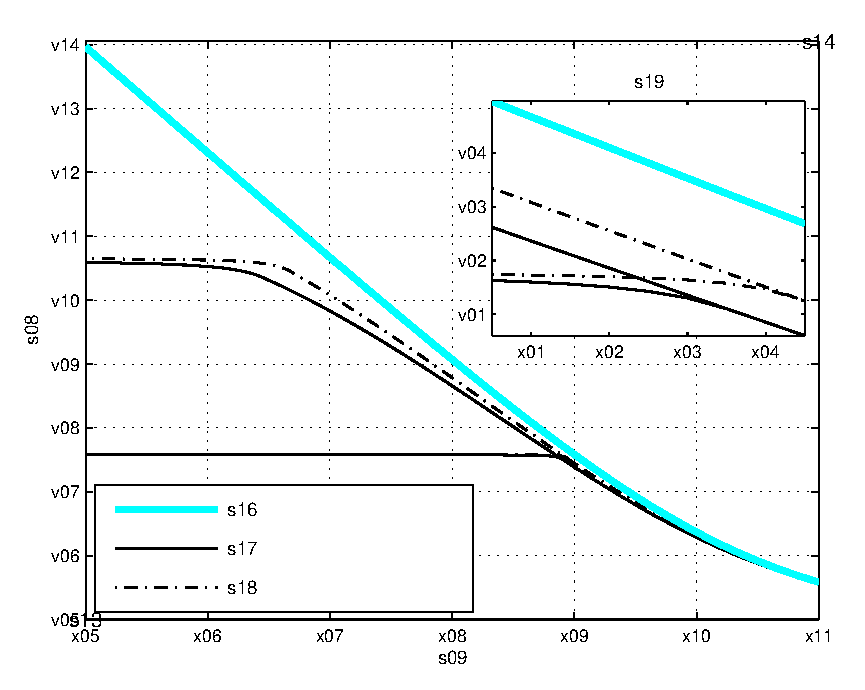
\includegraphics{fig_opt_thr_vs_SNR_AWGN.eps}}%
%\end{psfrags}%
%
% End fig_opt_thr_vs_SNR_AWGN.tex
\end{document}
% See http://www.mathworks.de/matlabcentral/fileexchange/loadFile.do?objectId=4638
% for recent versions of laprint.m.
%
% created by:           LaPrint version 3.16 (13.9.2004)
% created on:           13-Dec-2015 21:43:34
% eps bounding box:     16 cm x 12 cm
% comment:              
%
%\begin{psfrags}%
%\psfragscanon%
%
% text strings:
\psfrag{s08}[b][b]{\fontsize{8.5}{12.75}\fontseries{m}\mathversion{normal}\fontshape{n}\selectfont \color[rgb]{0,0,0}\setlength{\tabcolsep}{0pt}\begin{tabular}{c}$\rs(\ttau)$ [bits/sec/Hz]\end{tabular}}%
\psfrag{s09}[t][t]{\fontsize{8.5}{12.75}\fontseries{m}\mathversion{normal}\fontshape{n}\selectfont \color[rgb]{0,0,0}\setlength{\tabcolsep}{0pt}\begin{tabular}{c}$\gamma$ [dB]\end{tabular}}%
\psfrag{s13}[][]{\fontsize{10}{15}\fontseries{m}\mathversion{normal}\fontshape{n}\selectfont \color[rgb]{0,0,0}\setlength{\tabcolsep}{0pt}\begin{tabular}{c} \end{tabular}}%
\psfrag{s14}[][]{\fontsize{10}{15}\fontseries{m}\mathversion{normal}\fontshape{n}\selectfont \color[rgb]{0,0,0}\setlength{\tabcolsep}{0pt}\begin{tabular}{c} \end{tabular}}%
\psfrag{s15}[l][l]{\fontsize{8.5}{12.75}\fontseries{m}\mathversion{normal}\fontshape{n}\selectfont \color[rgb]{0,0,0}EM, $\opc = 0.1$}%
\psfrag{s16}[l][l]{\fontsize{8.5}{12.75}\fontseries{m}\mathversion{normal}\fontshape{n}\selectfont \color[rgb]{0,0,0}IM}%
\psfrag{s17}[l][l]{\fontsize{8.5}{12.75}\fontseries{m}\mathversion{normal}\fontshape{n}\selectfont \color[rgb]{0,0,0}EM, $\opc = 0.01$}%
\psfrag{s18}[l][l]{\fontsize{8.5}{12.75}\fontseries{m}\mathversion{normal}\fontshape{n}\selectfont \color[rgb]{0,0,0}EM, $\opc = 0.1$}%
\psfrag{s19}[b][b]{\fontsize{8.5}{12.75}\fontseries{m}\mathversion{normal}\fontshape{n}\selectfont \color[rgb]{0,0,0}\setlength{\tabcolsep}{0pt}\begin{tabular}{c}Zoom\end{tabular}}%
%
% axes font properties:
\fontsize{8.5}{12.75}\fontseries{m}\mathversion{normal}%
\fontshape{n}\selectfont%
%
% xticklabels:
\psfrag{x01}[t][t]{-1}%
\psfrag{x02}[t][t]{-0.8}%
\psfrag{x03}[t][t]{-0.6}%
\psfrag{x04}[t][t]{-0.4}%
\psfrag{x05}[t][t]{-20}%
\psfrag{x06}[t][t]{-15}%
\psfrag{x07}[t][t]{-10}%
\psfrag{x08}[t][t]{-5}%
\psfrag{x09}[t][t]{0}%
\psfrag{x10}[t][t]{5}%
\psfrag{x11}[t][t]{10}%
%
% yticklabels:
\psfrag{v01}[r][r]{2.5}%
\psfrag{v02}[r][r]{2.6}%
\psfrag{v03}[r][r]{2.7}%
\psfrag{v04}[r][r]{2.8}%
\psfrag{v05}[r][r]{0}%
\psfrag{v06}[r][r]{1}%
\psfrag{v07}[r][r]{2}%
\psfrag{v08}[r][r]{3}%
\psfrag{v09}[r][r]{4}%
\psfrag{v10}[r][r]{5}%
\psfrag{v11}[r][r]{6}%
\psfrag{v12}[r][r]{7}%
\psfrag{v13}[r][r]{8}%
\psfrag{v14}[r][r]{9}%
%
% Figure:
%\resizebox{8cm}{!}{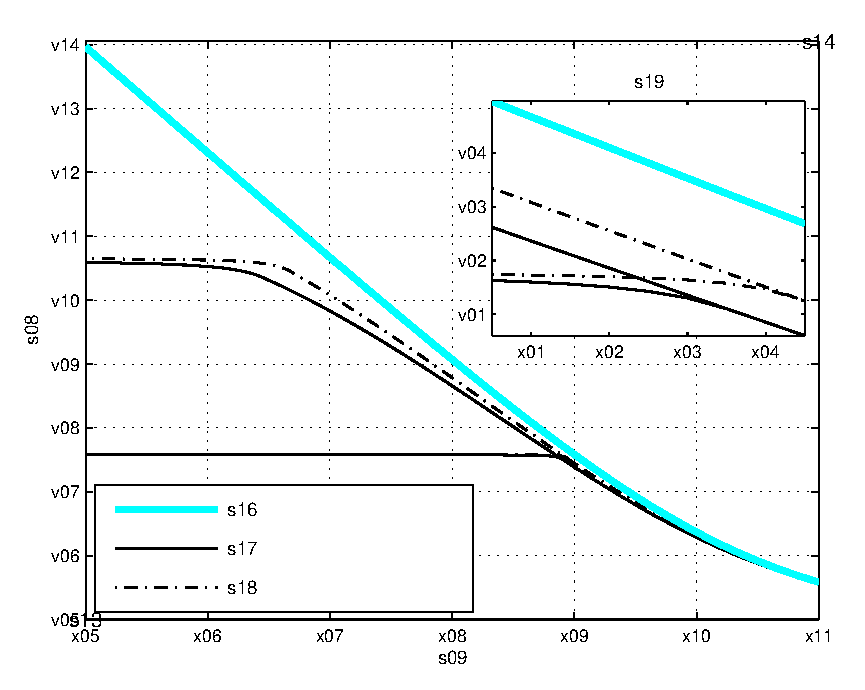
\includegraphics{fig_opt_thr_vs_SNR_AWGN.eps}}%
%\end{psfrags}%
%
% End fig_opt_thr_vs_SNR_AWGN.tex
\end{document}
% See http://www.mathworks.de/matlabcentral/fileexchange/loadFile.do?objectId=4638
% for recent versions of laprint.m.
%
% created by:           LaPrint version 3.16 (13.9.2004)
% created on:           13-Dec-2015 21:43:34
% eps bounding box:     16 cm x 12 cm
% comment:              
%
%\begin{psfrags}%
%\psfragscanon%
%
% text strings:
\psfrag{s08}[b][b]{\fontsize{8.5}{12.75}\fontseries{m}\mathversion{normal}\fontshape{n}\selectfont \color[rgb]{0,0,0}\setlength{\tabcolsep}{0pt}\begin{tabular}{c}$\rs(\ttau)$ [bits/sec/Hz]\end{tabular}}%
\psfrag{s09}[t][t]{\fontsize{8.5}{12.75}\fontseries{m}\mathversion{normal}\fontshape{n}\selectfont \color[rgb]{0,0,0}\setlength{\tabcolsep}{0pt}\begin{tabular}{c}$\gamma$ [dB]\end{tabular}}%
\psfrag{s13}[][]{\fontsize{10}{15}\fontseries{m}\mathversion{normal}\fontshape{n}\selectfont \color[rgb]{0,0,0}\setlength{\tabcolsep}{0pt}\begin{tabular}{c} \end{tabular}}%
\psfrag{s14}[][]{\fontsize{10}{15}\fontseries{m}\mathversion{normal}\fontshape{n}\selectfont \color[rgb]{0,0,0}\setlength{\tabcolsep}{0pt}\begin{tabular}{c} \end{tabular}}%
\psfrag{s15}[l][l]{\fontsize{8.5}{12.75}\fontseries{m}\mathversion{normal}\fontshape{n}\selectfont \color[rgb]{0,0,0}EM, $\opc = 0.1$}%
\psfrag{s16}[l][l]{\fontsize{8.5}{12.75}\fontseries{m}\mathversion{normal}\fontshape{n}\selectfont \color[rgb]{0,0,0}IM}%
\psfrag{s17}[l][l]{\fontsize{8.5}{12.75}\fontseries{m}\mathversion{normal}\fontshape{n}\selectfont \color[rgb]{0,0,0}EM, $\opc = 0.01$}%
\psfrag{s18}[l][l]{\fontsize{8.5}{12.75}\fontseries{m}\mathversion{normal}\fontshape{n}\selectfont \color[rgb]{0,0,0}EM, $\opc = 0.1$}%
\psfrag{s19}[b][b]{\fontsize{8.5}{12.75}\fontseries{m}\mathversion{normal}\fontshape{n}\selectfont \color[rgb]{0,0,0}\setlength{\tabcolsep}{0pt}\begin{tabular}{c}Zoom\end{tabular}}%
%
% axes font properties:
\fontsize{8.5}{12.75}\fontseries{m}\mathversion{normal}%
\fontshape{n}\selectfont%
%
% xticklabels:
\psfrag{x01}[t][t]{-1}%
\psfrag{x02}[t][t]{-0.8}%
\psfrag{x03}[t][t]{-0.6}%
\psfrag{x04}[t][t]{-0.4}%
\psfrag{x05}[t][t]{-20}%
\psfrag{x06}[t][t]{-15}%
\psfrag{x07}[t][t]{-10}%
\psfrag{x08}[t][t]{-5}%
\psfrag{x09}[t][t]{0}%
\psfrag{x10}[t][t]{5}%
\psfrag{x11}[t][t]{10}%
%
% yticklabels:
\psfrag{v01}[r][r]{2.5}%
\psfrag{v02}[r][r]{2.6}%
\psfrag{v03}[r][r]{2.7}%
\psfrag{v04}[r][r]{2.8}%
\psfrag{v05}[r][r]{0}%
\psfrag{v06}[r][r]{1}%
\psfrag{v07}[r][r]{2}%
\psfrag{v08}[r][r]{3}%
\psfrag{v09}[r][r]{4}%
\psfrag{v10}[r][r]{5}%
\psfrag{v11}[r][r]{6}%
\psfrag{v12}[r][r]{7}%
\psfrag{v13}[r][r]{8}%
\psfrag{v14}[r][r]{9}%
%
% Figure:
%\resizebox{8cm}{!}{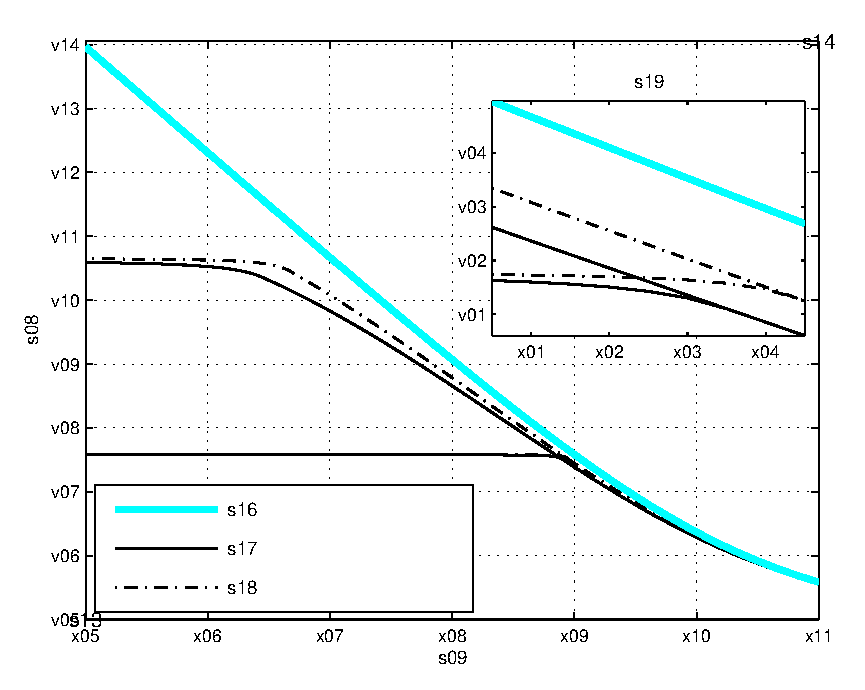
\includegraphics{fig_opt_thr_vs_SNR_AWGN.eps}}%
%\end{psfrags}%
%
% End fig_opt_thr_vs_SNR_AWGN.tex
\end{document}
% See http://www.mathworks.de/matlabcentral/fileexchange/loadFile.do?objectId=4638
% for recent versions of laprint.m.
%
% created by:           LaPrint version 3.16 (13.9.2004)
% created on:           13-Dec-2015 21:43:34
% eps bounding box:     16 cm x 12 cm
% comment:              
%
%\begin{psfrags}%
%\psfragscanon%
%
% text strings:
\psfrag{s08}[b][b]{\fontsize{8.5}{12.75}\fontseries{m}\mathversion{normal}\fontshape{n}\selectfont \color[rgb]{0,0,0}\setlength{\tabcolsep}{0pt}\begin{tabular}{c}$\rs(\ttau)$ [bits/sec/Hz]\end{tabular}}%
\psfrag{s09}[t][t]{\fontsize{8.5}{12.75}\fontseries{m}\mathversion{normal}\fontshape{n}\selectfont \color[rgb]{0,0,0}\setlength{\tabcolsep}{0pt}\begin{tabular}{c}$\gamma$ [dB]\end{tabular}}%
\psfrag{s13}[][]{\fontsize{10}{15}\fontseries{m}\mathversion{normal}\fontshape{n}\selectfont \color[rgb]{0,0,0}\setlength{\tabcolsep}{0pt}\begin{tabular}{c} \end{tabular}}%
\psfrag{s14}[][]{\fontsize{10}{15}\fontseries{m}\mathversion{normal}\fontshape{n}\selectfont \color[rgb]{0,0,0}\setlength{\tabcolsep}{0pt}\begin{tabular}{c} \end{tabular}}%
\psfrag{s15}[l][l]{\fontsize{8.5}{12.75}\fontseries{m}\mathversion{normal}\fontshape{n}\selectfont \color[rgb]{0,0,0}EM, $\opc = 0.1$}%
\psfrag{s16}[l][l]{\fontsize{8.5}{12.75}\fontseries{m}\mathversion{normal}\fontshape{n}\selectfont \color[rgb]{0,0,0}IM}%
\psfrag{s17}[l][l]{\fontsize{8.5}{12.75}\fontseries{m}\mathversion{normal}\fontshape{n}\selectfont \color[rgb]{0,0,0}EM, $\opc = 0.01$}%
\psfrag{s18}[l][l]{\fontsize{8.5}{12.75}\fontseries{m}\mathversion{normal}\fontshape{n}\selectfont \color[rgb]{0,0,0}EM, $\opc = 0.1$}%
\psfrag{s19}[b][b]{\fontsize{8.5}{12.75}\fontseries{m}\mathversion{normal}\fontshape{n}\selectfont \color[rgb]{0,0,0}\setlength{\tabcolsep}{0pt}\begin{tabular}{c}Zoom\end{tabular}}%
%
% axes font properties:
\fontsize{8.5}{12.75}\fontseries{m}\mathversion{normal}%
\fontshape{n}\selectfont%
%
% xticklabels:
\psfrag{x01}[t][t]{-1}%
\psfrag{x02}[t][t]{-0.8}%
\psfrag{x03}[t][t]{-0.6}%
\psfrag{x04}[t][t]{-0.4}%
\psfrag{x05}[t][t]{-20}%
\psfrag{x06}[t][t]{-15}%
\psfrag{x07}[t][t]{-10}%
\psfrag{x08}[t][t]{-5}%
\psfrag{x09}[t][t]{0}%
\psfrag{x10}[t][t]{5}%
\psfrag{x11}[t][t]{10}%
%
% yticklabels:
\psfrag{v01}[r][r]{2.5}%
\psfrag{v02}[r][r]{2.6}%
\psfrag{v03}[r][r]{2.7}%
\psfrag{v04}[r][r]{2.8}%
\psfrag{v05}[r][r]{0}%
\psfrag{v06}[r][r]{1}%
\psfrag{v07}[r][r]{2}%
\psfrag{v08}[r][r]{3}%
\psfrag{v09}[r][r]{4}%
\psfrag{v10}[r][r]{5}%
\psfrag{v11}[r][r]{6}%
\psfrag{v12}[r][r]{7}%
\psfrag{v13}[r][r]{8}%
\psfrag{v14}[r][r]{9}%
%
% Figure:
%\resizebox{8cm}{!}{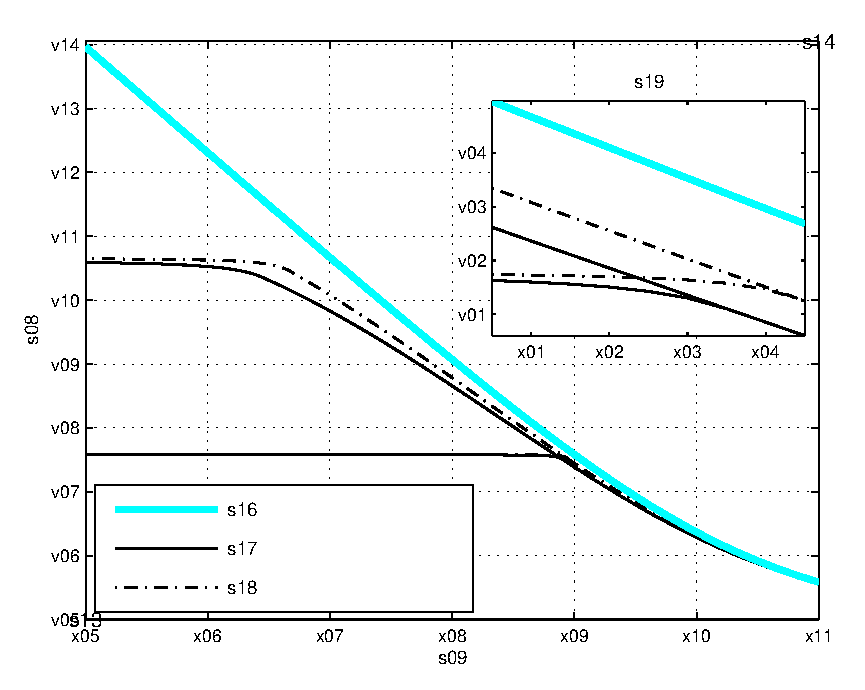
\includegraphics{fig_opt_thr_vs_SNR_AWGN.eps}}%
%\end{psfrags}%
%
% End fig_opt_thr_vs_SNR_AWGN.tex
